\movedhead{Response variability}
\label{sec:variability}\label{app:variability}
Because \texttt{temperature} cannot be set on these models, repeated sampling
replaces it and the resulting variability is reported as a result rather than
treated as nuisance. Mean within-item entropy across five identical prompts
separates the models more sharply than effort does: Opus sits between 0.057
and 0.147 bits, Sonnet between 0.053 and 0.311, and Haiku between 0.354 and
0.510. The within-item share of variance in the continuous measure runs from
4.5\% in Sonnet at \texttt{low} effort to 33.6\% in Haiku at \texttt{high}.
Most variance is between items, which is what an instrument that measures its
stimulus should show, but a third of it is within item in Haiku, so a single
sample per item would have been closer to a coin flip than to a measurement.

The pre-registration singles out one combination as the worst outcome for
deployment: an effect size that does not move while entropy falls, which
would mean the model becoming more confident in the same biased answer. It
does not occur. In Haiku and Sonnet entropy rises with effort, from 0.354 to
0.479 and from 0.054 to 0.311, while their absolute effects fall or hold. In
Opus entropy does fall, from 0.147 at \texttt{low} to 0.060 at
\texttt{high}, but its absolute effect falls with it and is the one pooled
slope whose interval excludes zero, so the rising confidence attaches to a
less biased answer rather than to the same one.

\begin{figure}[t]
  \centering
  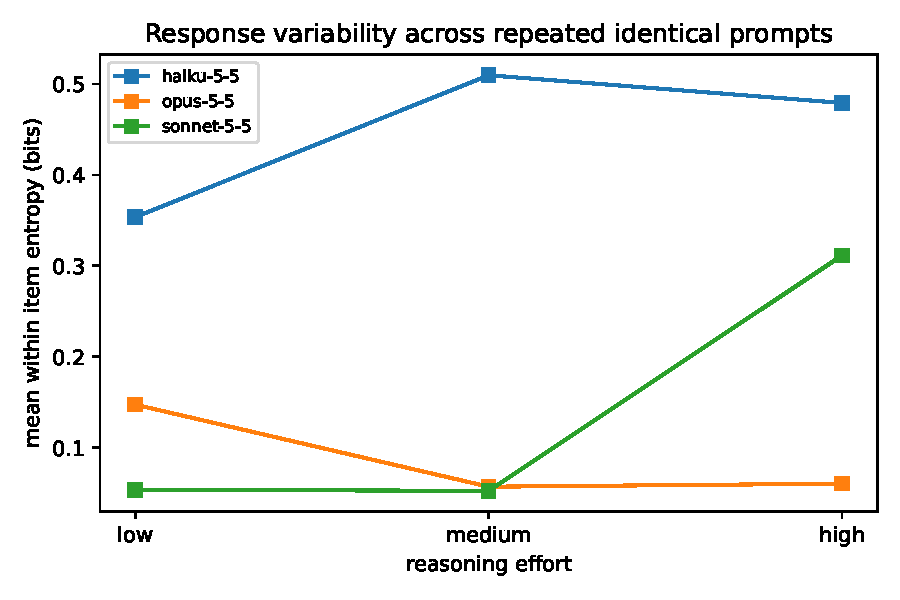
\includegraphics[width=0.7\linewidth]{../figures/fig3_entropy.pdf}
  \caption{Within-item entropy across five identical repeated prompts.}
  \label{fig:entropy}
\end{figure}
